% Options for packages loaded elsewhere
\PassOptionsToPackage{unicode}{hyperref}
\PassOptionsToPackage{hyphens}{url}
%
\documentclass[
]{article}
\usepackage{amsmath,amssymb}
\usepackage{lmodern}
\usepackage{iftex}
\ifPDFTeX
  \usepackage[T1]{fontenc}
  \usepackage[utf8]{inputenc}
  \usepackage{textcomp} % provide euro and other symbols
\else % if luatex or xetex
  \usepackage{unicode-math}
  \defaultfontfeatures{Scale=MatchLowercase}
  \defaultfontfeatures[\rmfamily]{Ligatures=TeX,Scale=1}
\fi
% Use upquote if available, for straight quotes in verbatim environments
\IfFileExists{upquote.sty}{\usepackage{upquote}}{}
\IfFileExists{microtype.sty}{% use microtype if available
  \usepackage[]{microtype}
  \UseMicrotypeSet[protrusion]{basicmath} % disable protrusion for tt fonts
}{}
\makeatletter
\@ifundefined{KOMAClassName}{% if non-KOMA class
  \IfFileExists{parskip.sty}{%
    \usepackage{parskip}
  }{% else
    \setlength{\parindent}{0pt}
    \setlength{\parskip}{6pt plus 2pt minus 1pt}}
}{% if KOMA class
  \KOMAoptions{parskip=half}}
\makeatother
\usepackage{xcolor}
\usepackage[margin=1in]{geometry}
\usepackage{graphicx}
\makeatletter
\def\maxwidth{\ifdim\Gin@nat@width>\linewidth\linewidth\else\Gin@nat@width\fi}
\def\maxheight{\ifdim\Gin@nat@height>\textheight\textheight\else\Gin@nat@height\fi}
\makeatother
% Scale images if necessary, so that they will not overflow the page
% margins by default, and it is still possible to overwrite the defaults
% using explicit options in \includegraphics[width, height, ...]{}
\setkeys{Gin}{width=\maxwidth,height=\maxheight,keepaspectratio}
% Set default figure placement to htbp
\makeatletter
\def\fps@figure{htbp}
\makeatother
\setlength{\emergencystretch}{3em} % prevent overfull lines
\providecommand{\tightlist}{%
  \setlength{\itemsep}{0pt}\setlength{\parskip}{0pt}}
\setcounter{secnumdepth}{-\maxdimen} % remove section numbering
\ifLuaTeX
  \usepackage{selnolig}  % disable illegal ligatures
\fi
\IfFileExists{bookmark.sty}{\usepackage{bookmark}}{\usepackage{hyperref}}
\IfFileExists{xurl.sty}{\usepackage{xurl}}{} % add URL line breaks if available
\urlstyle{same} % disable monospaced font for URLs
\hypersetup{
  pdftitle={report},
  hidelinks,
  pdfcreator={LaTeX via pandoc}}

\title{report}
\author{}
\date{\vspace{-2.5em}2022-10-28}

\begin{document}
\maketitle

\#\#Introduction

My project will use climatology data from three NOAA buoys near Cape
Hatteras, Duck, and Beaufort North Carolina to understand the trends in
water temperature, specifically in relation to gulf stream changes.
There was a heatwave in North Carolina in 2017 that may have been
amplified by a Gulf Stream warm core ring.

To test this, we can compare water temperature above the Gulf Stream
(Duck), at Gulf Stream shift (Cape Hatteras), and below the Gulf Stream
(Beaufort). In theory, if the Gulf stream did release a warm core ring,
there would be a rapid increase in temperature most likely starting at
the Duck buoy. We can also compare rates of warming between these three
locations and see the overall trends in water temperature on the NC
Coast.

These datasets have a variety of climate based variables including air
temperature, water temperature, wind speed, atmospheric pressure, and a
few other variables that may be of interest.

Measurements are taken every 6 minutes, and the dataset spans from 2016
to present day. To make these datasets easily usable, we will average
measurements each day.

Here are the figures I have so far :)

\#\#Figures

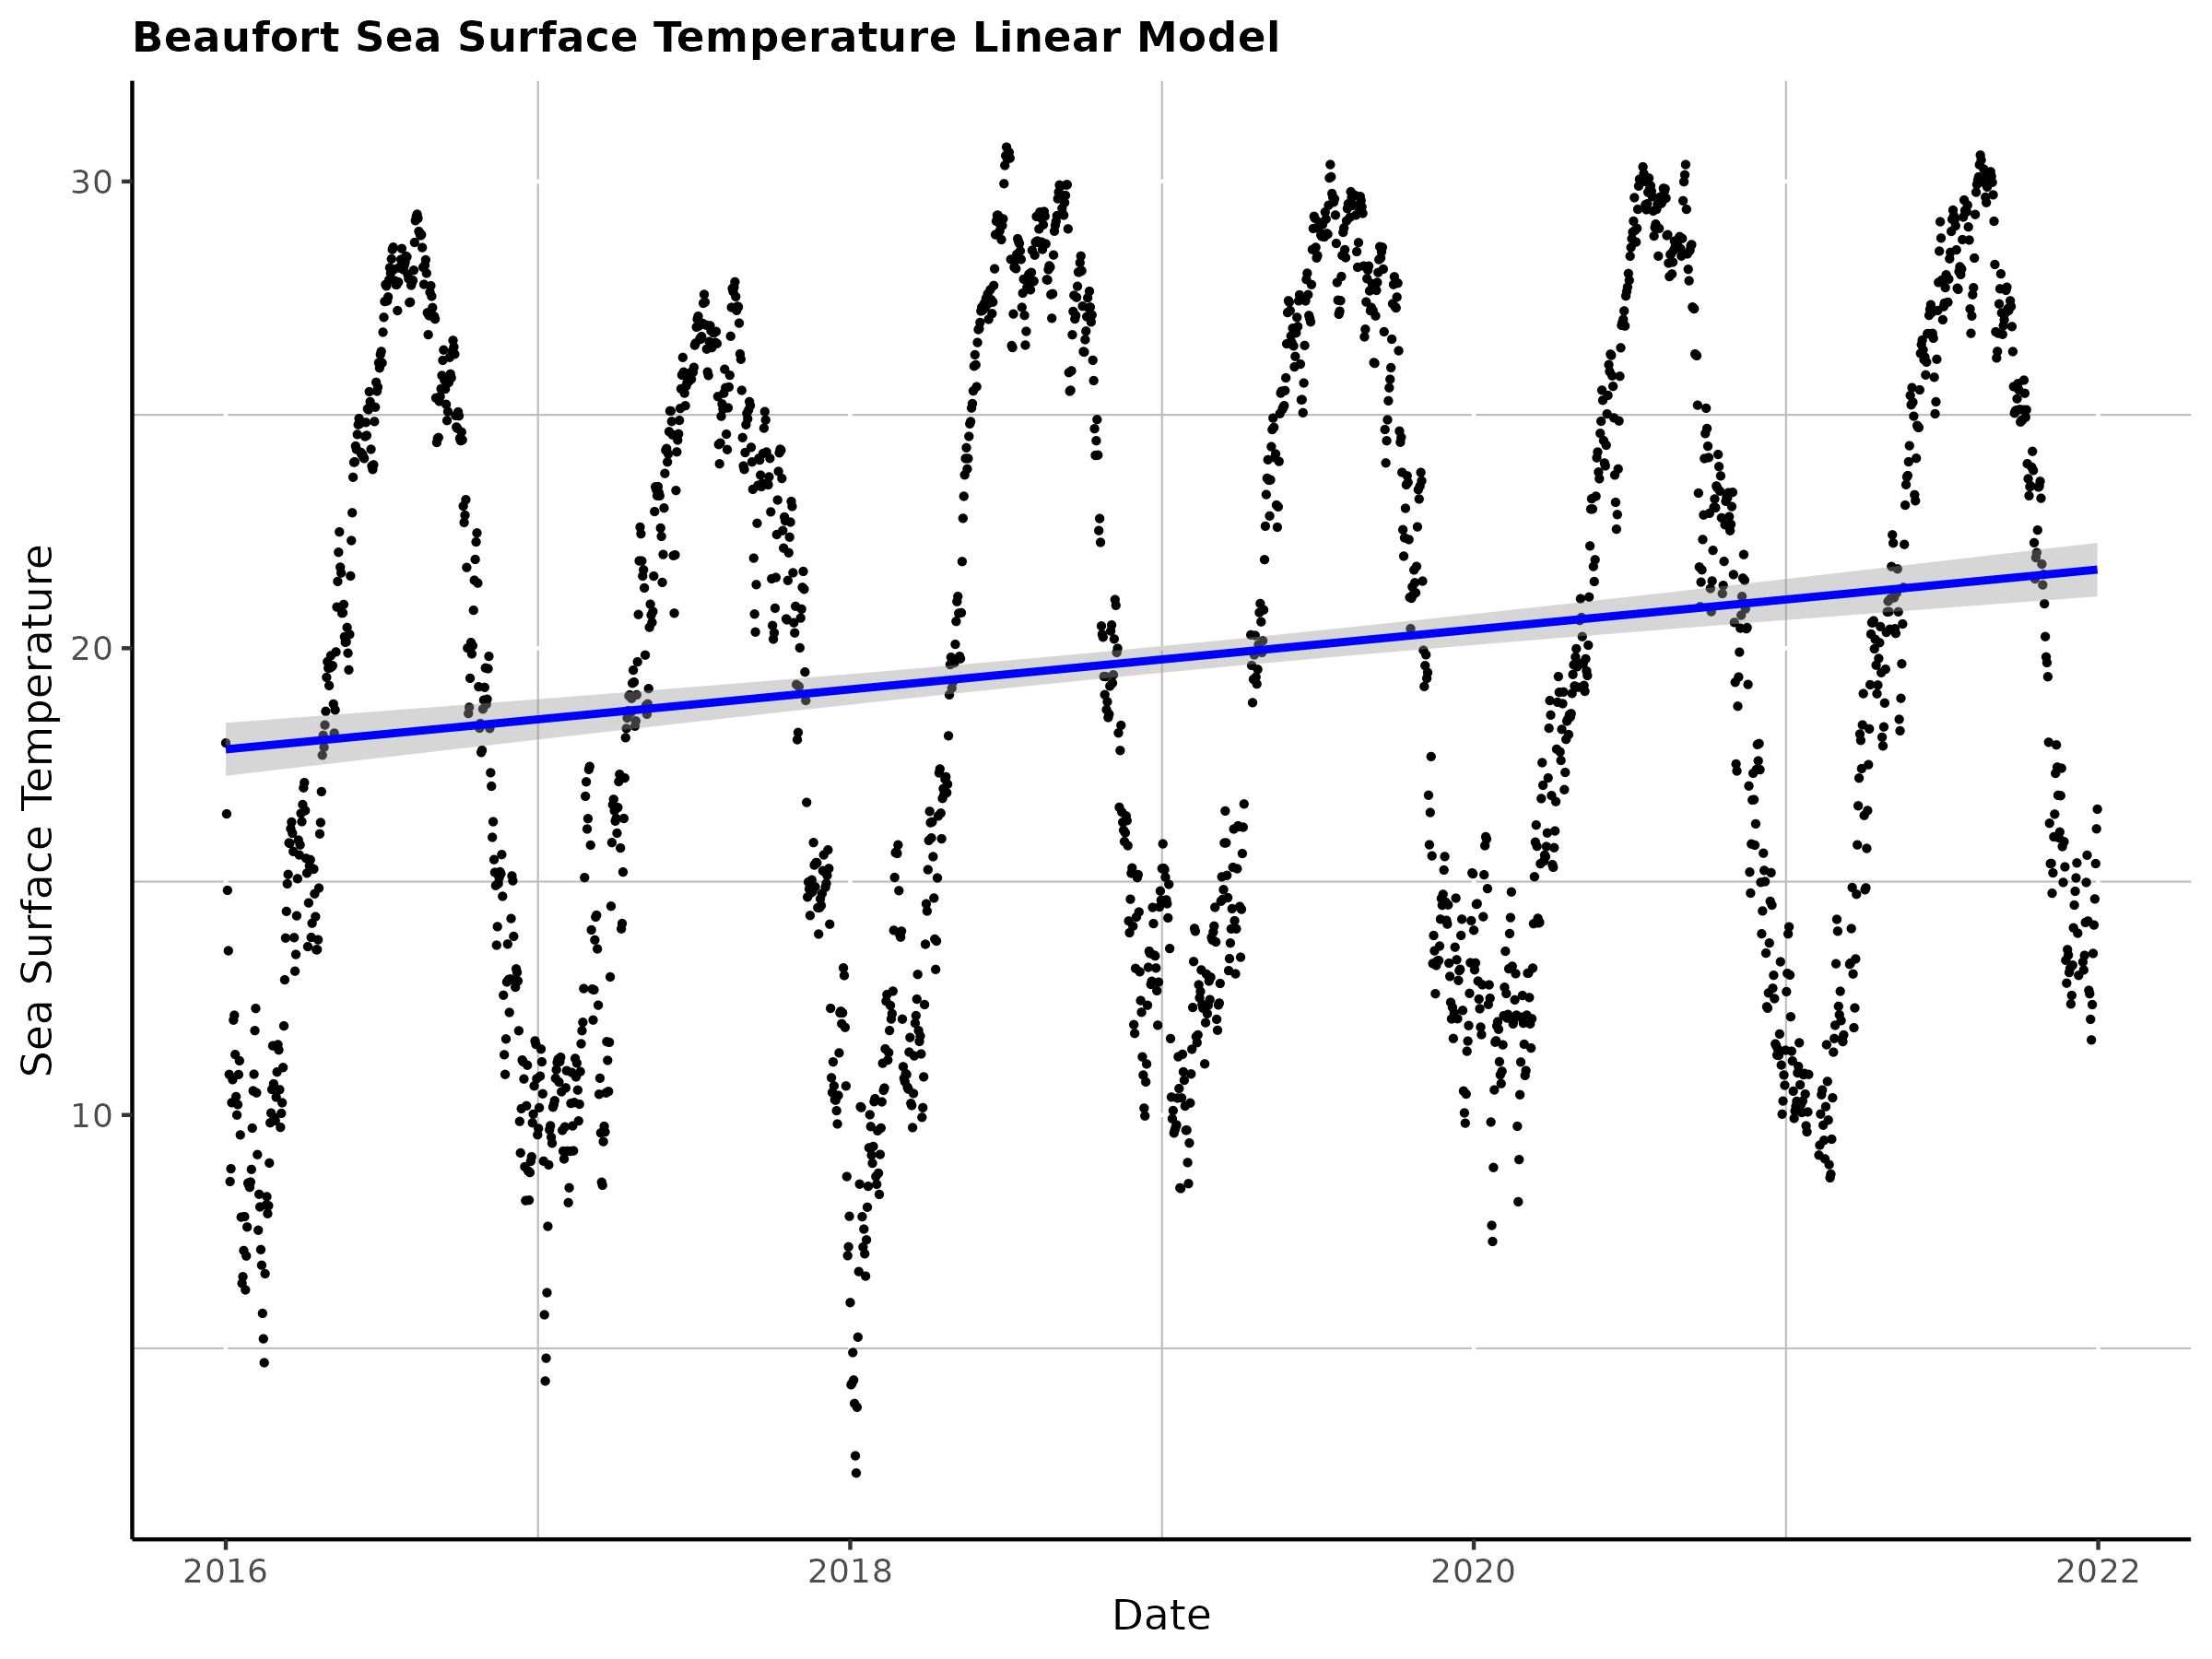
\includegraphics{figures/beaufsstglm.png}
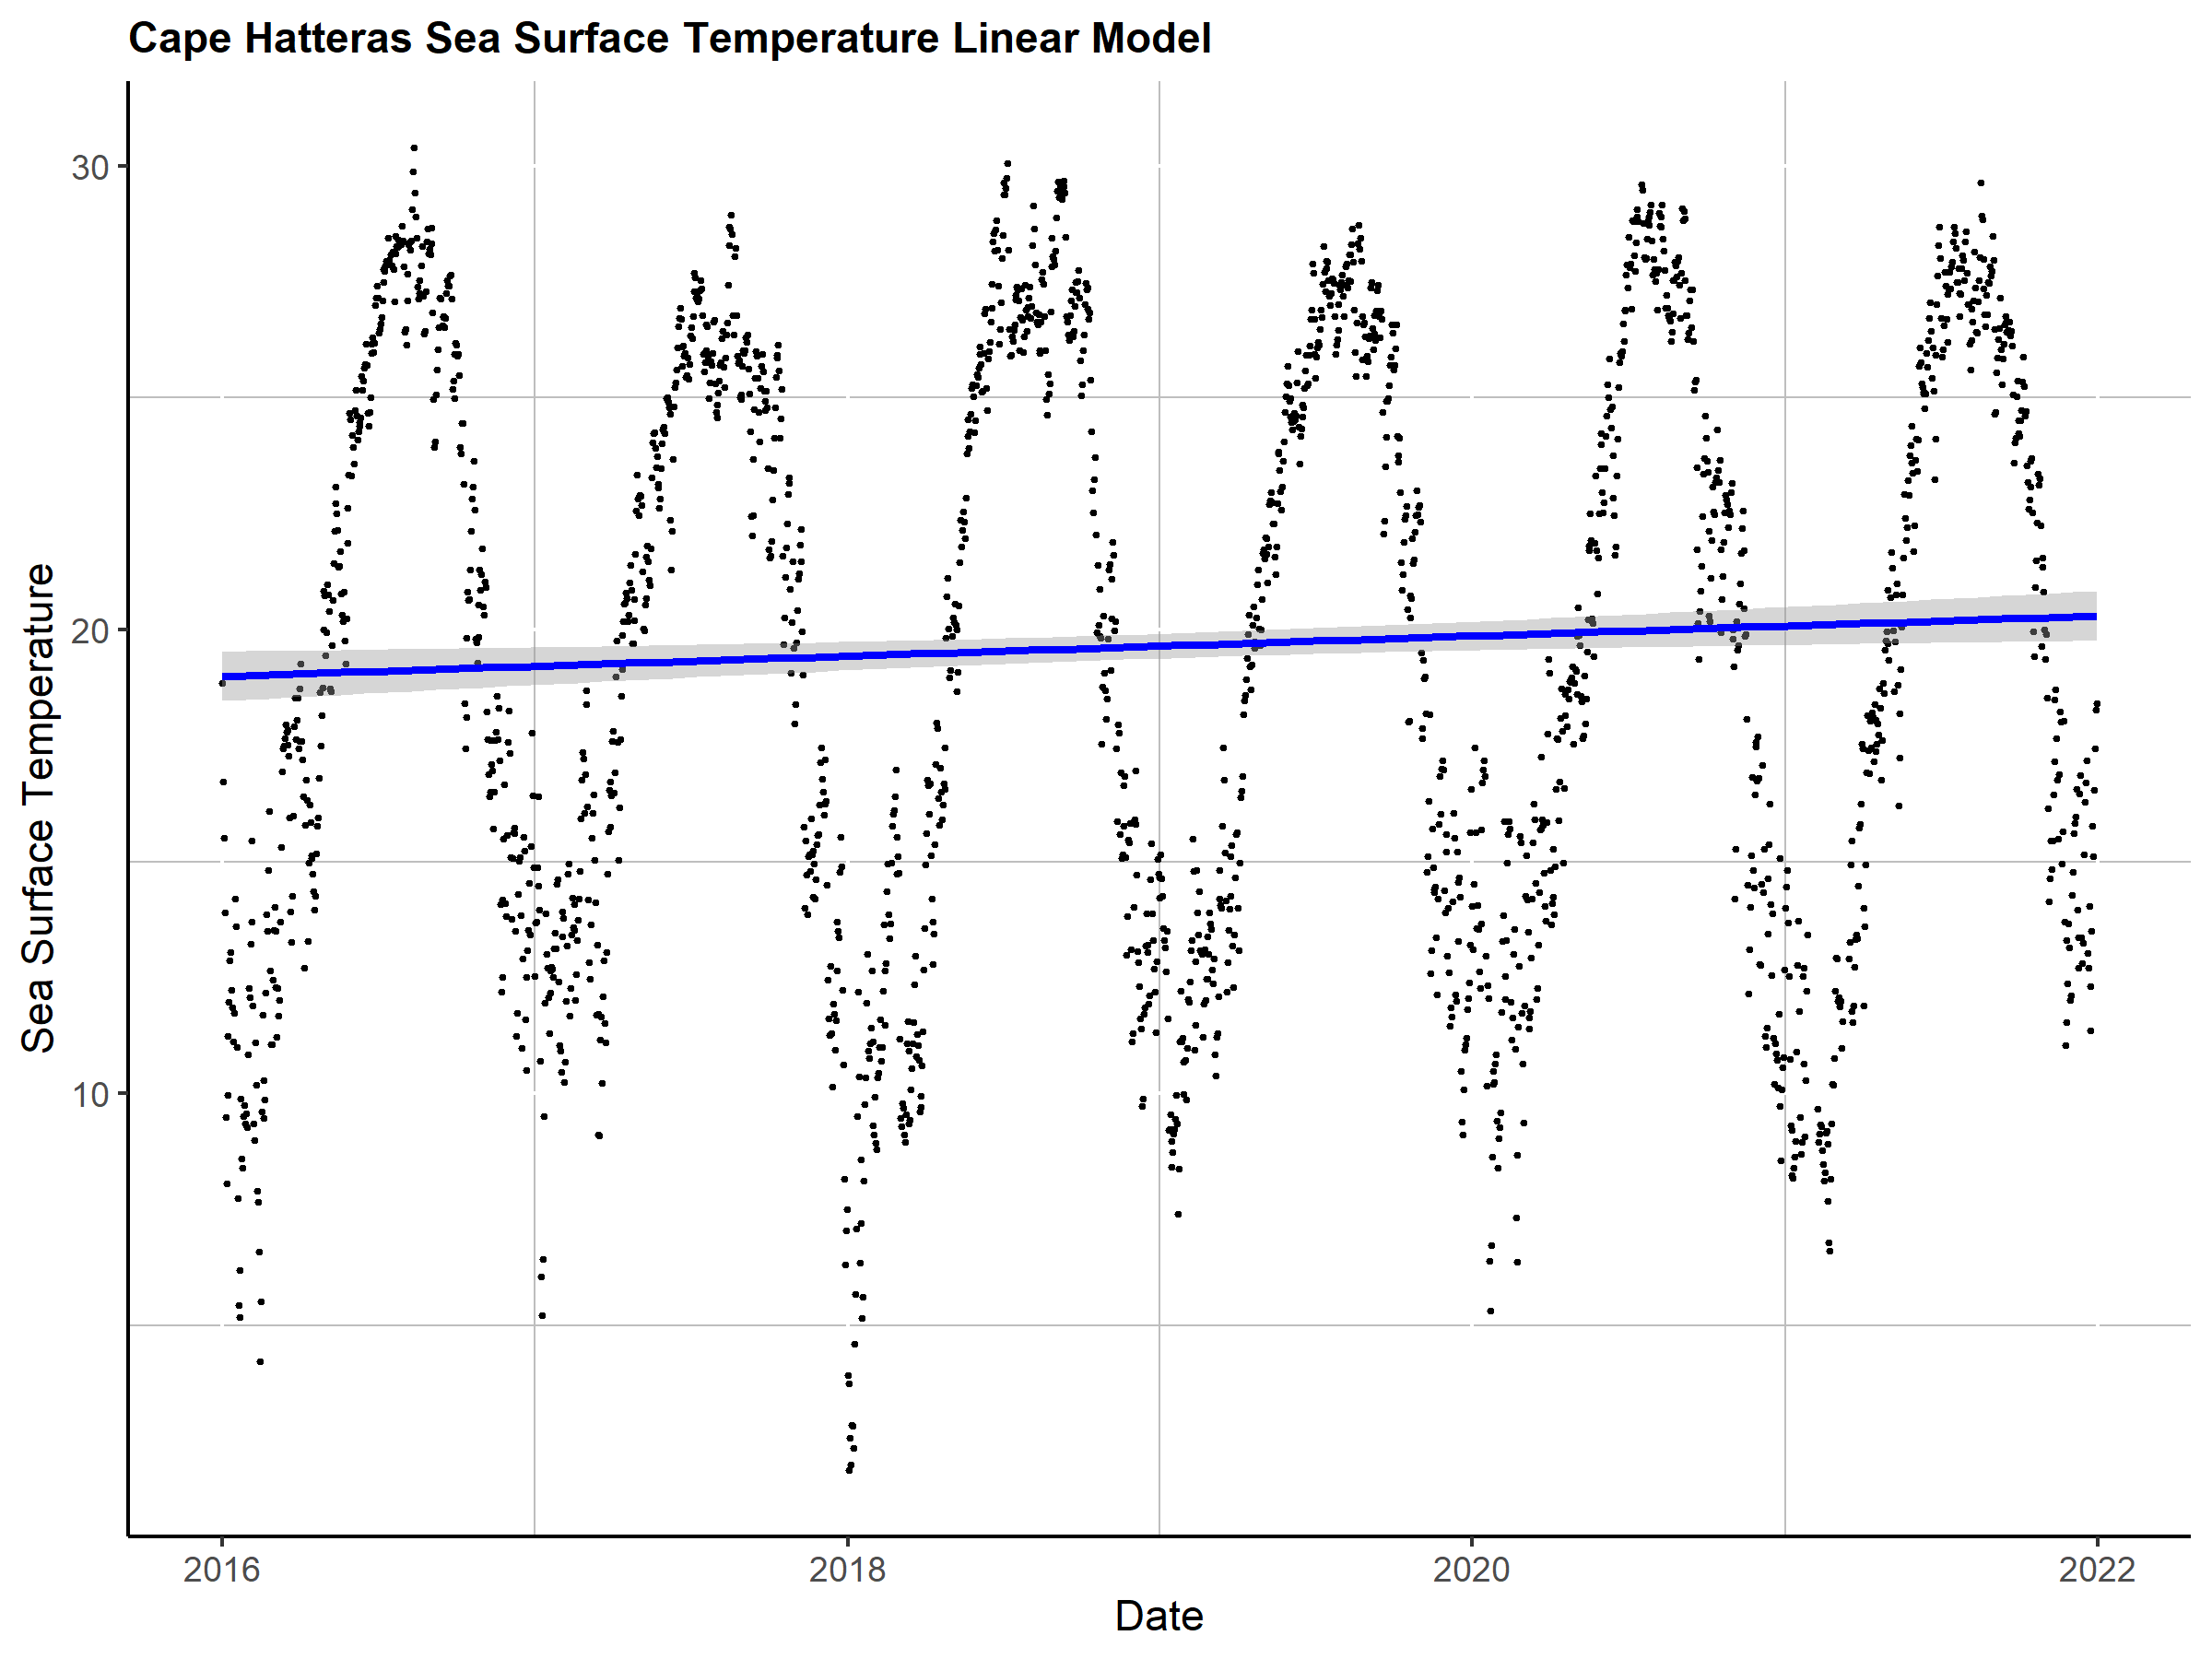
\includegraphics{figures/chsstglm.png}
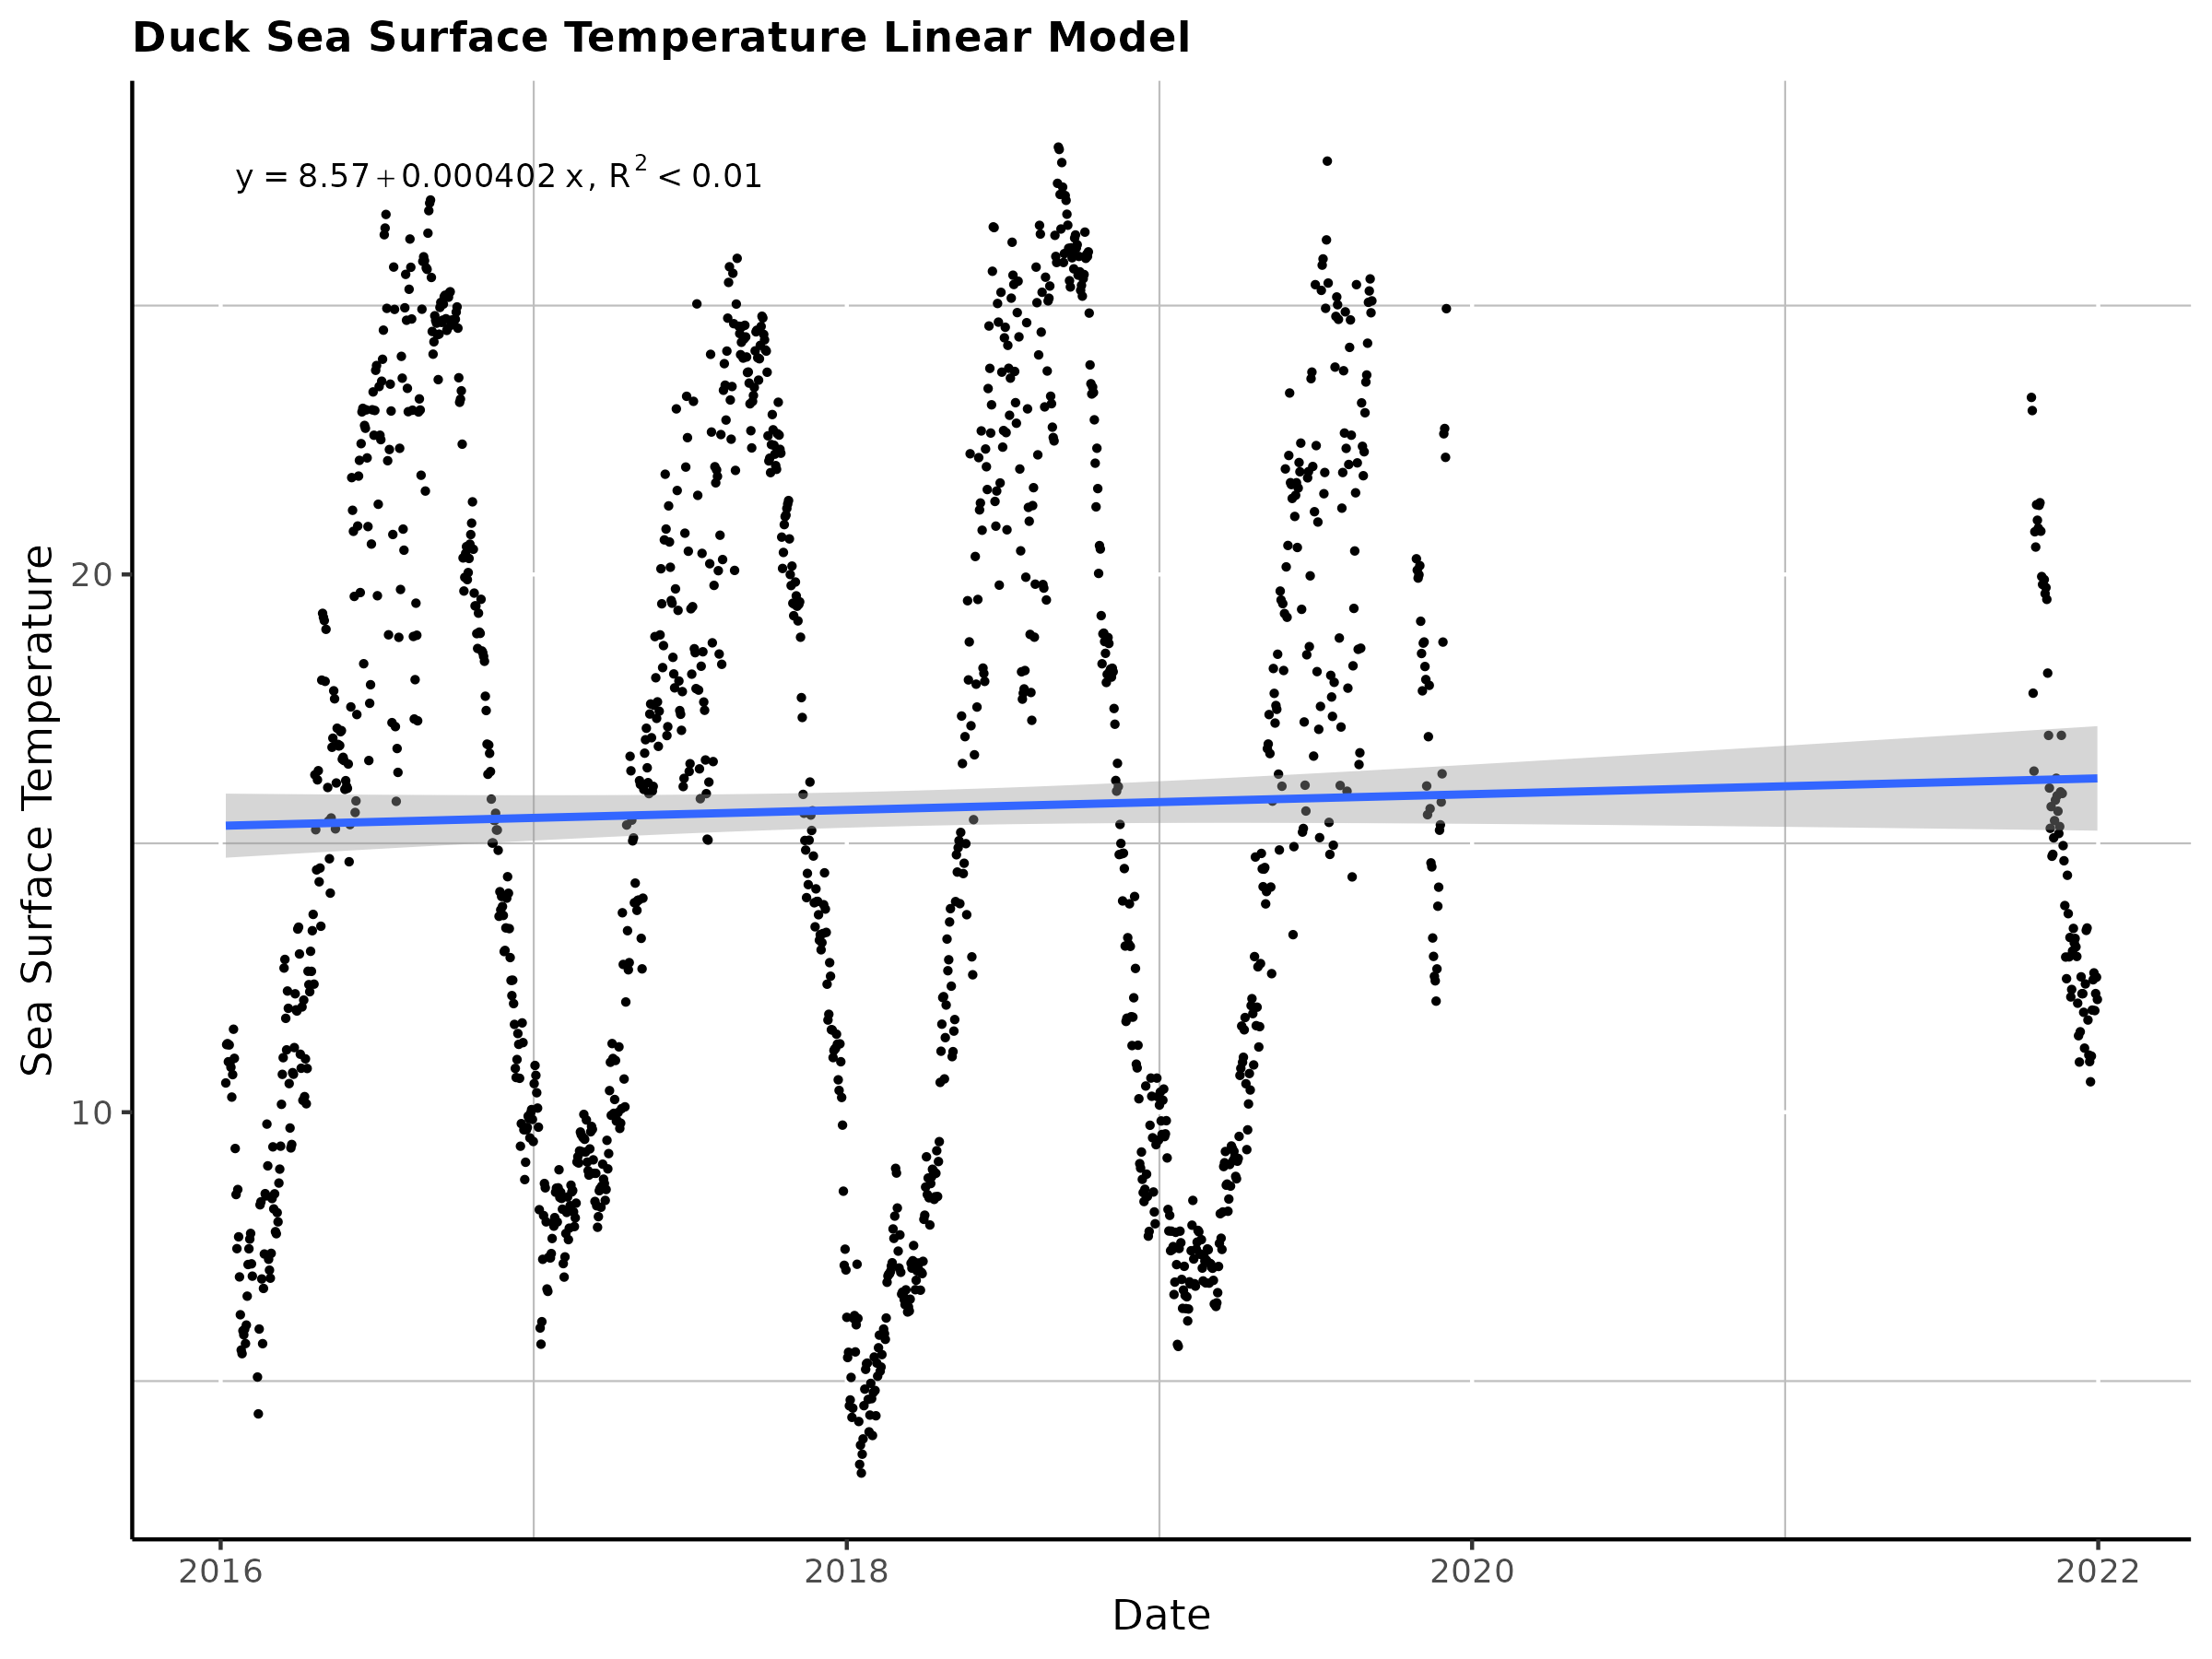
\includegraphics{figures/ducksstglm.png} Linear models for each buoy
site. It appears that Beaufort may have the most significant increase in
temperature over time.

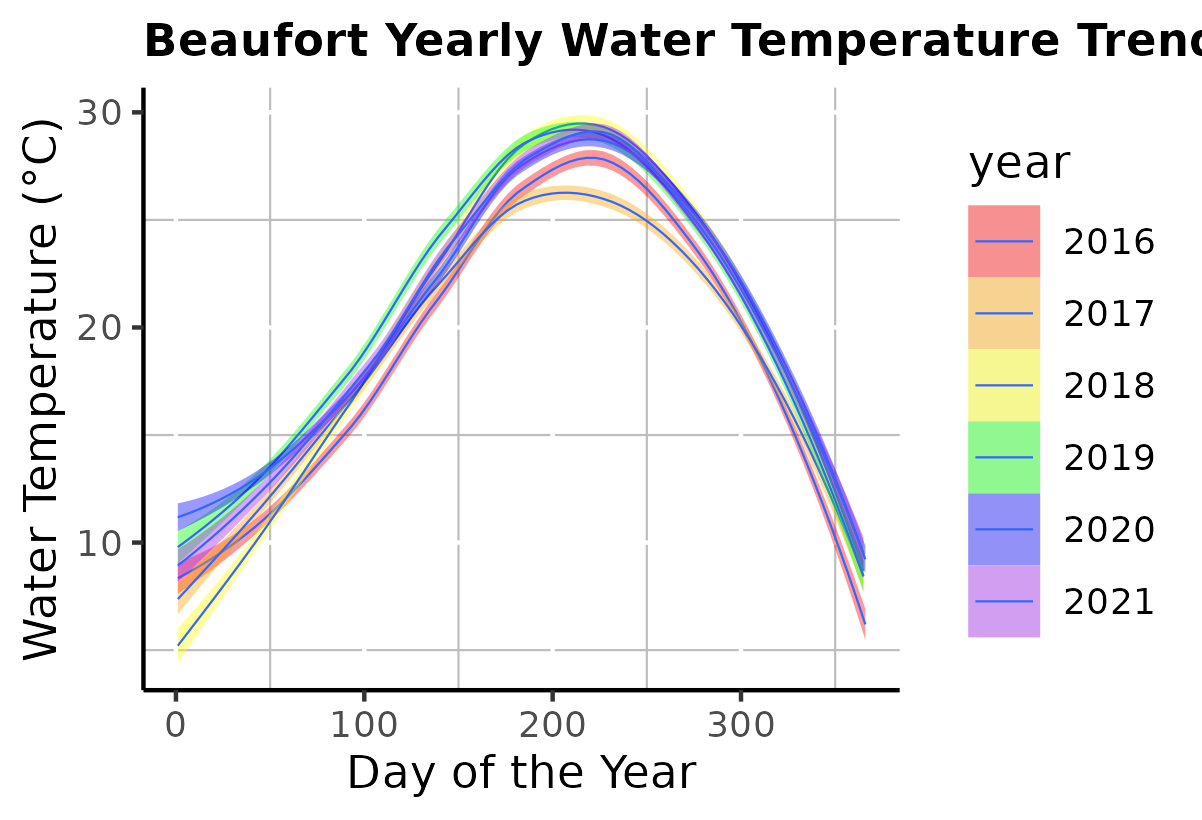
\includegraphics{figures/beaufyearlytrend.png}
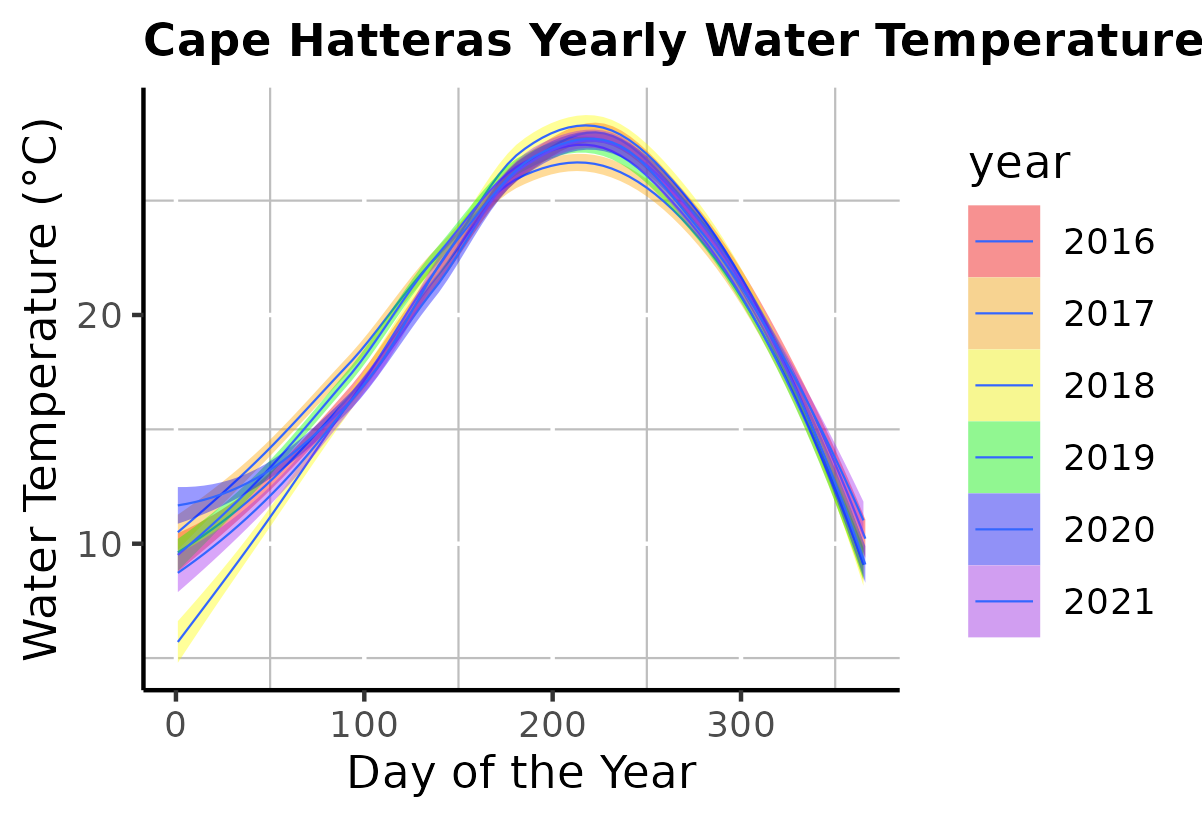
\includegraphics{figures/chyearlytrend.png}
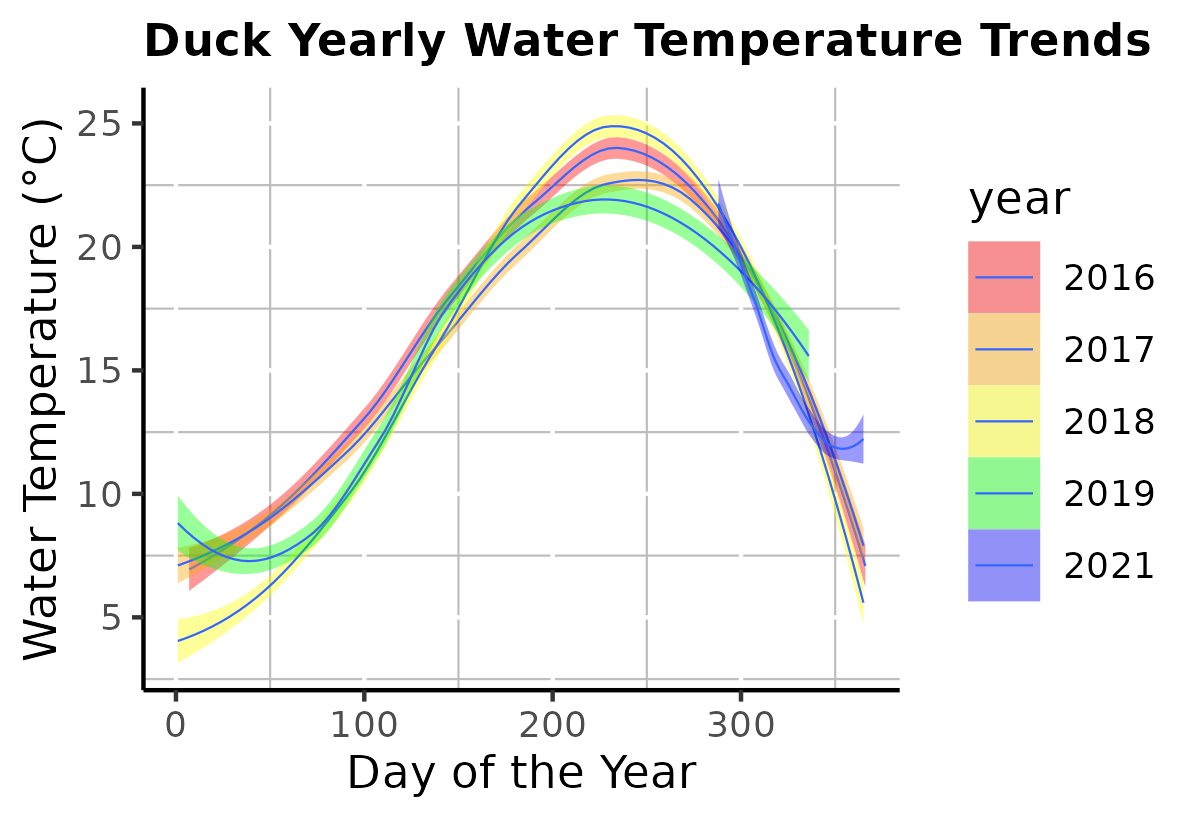
\includegraphics{figures/duckyearlytrend.png} Yearly trends for each
buoy site. Beaufort hits a much higher temperature than Cape Hatteras
and Duck. 2017 does not seem to be dramatically different than other
years.

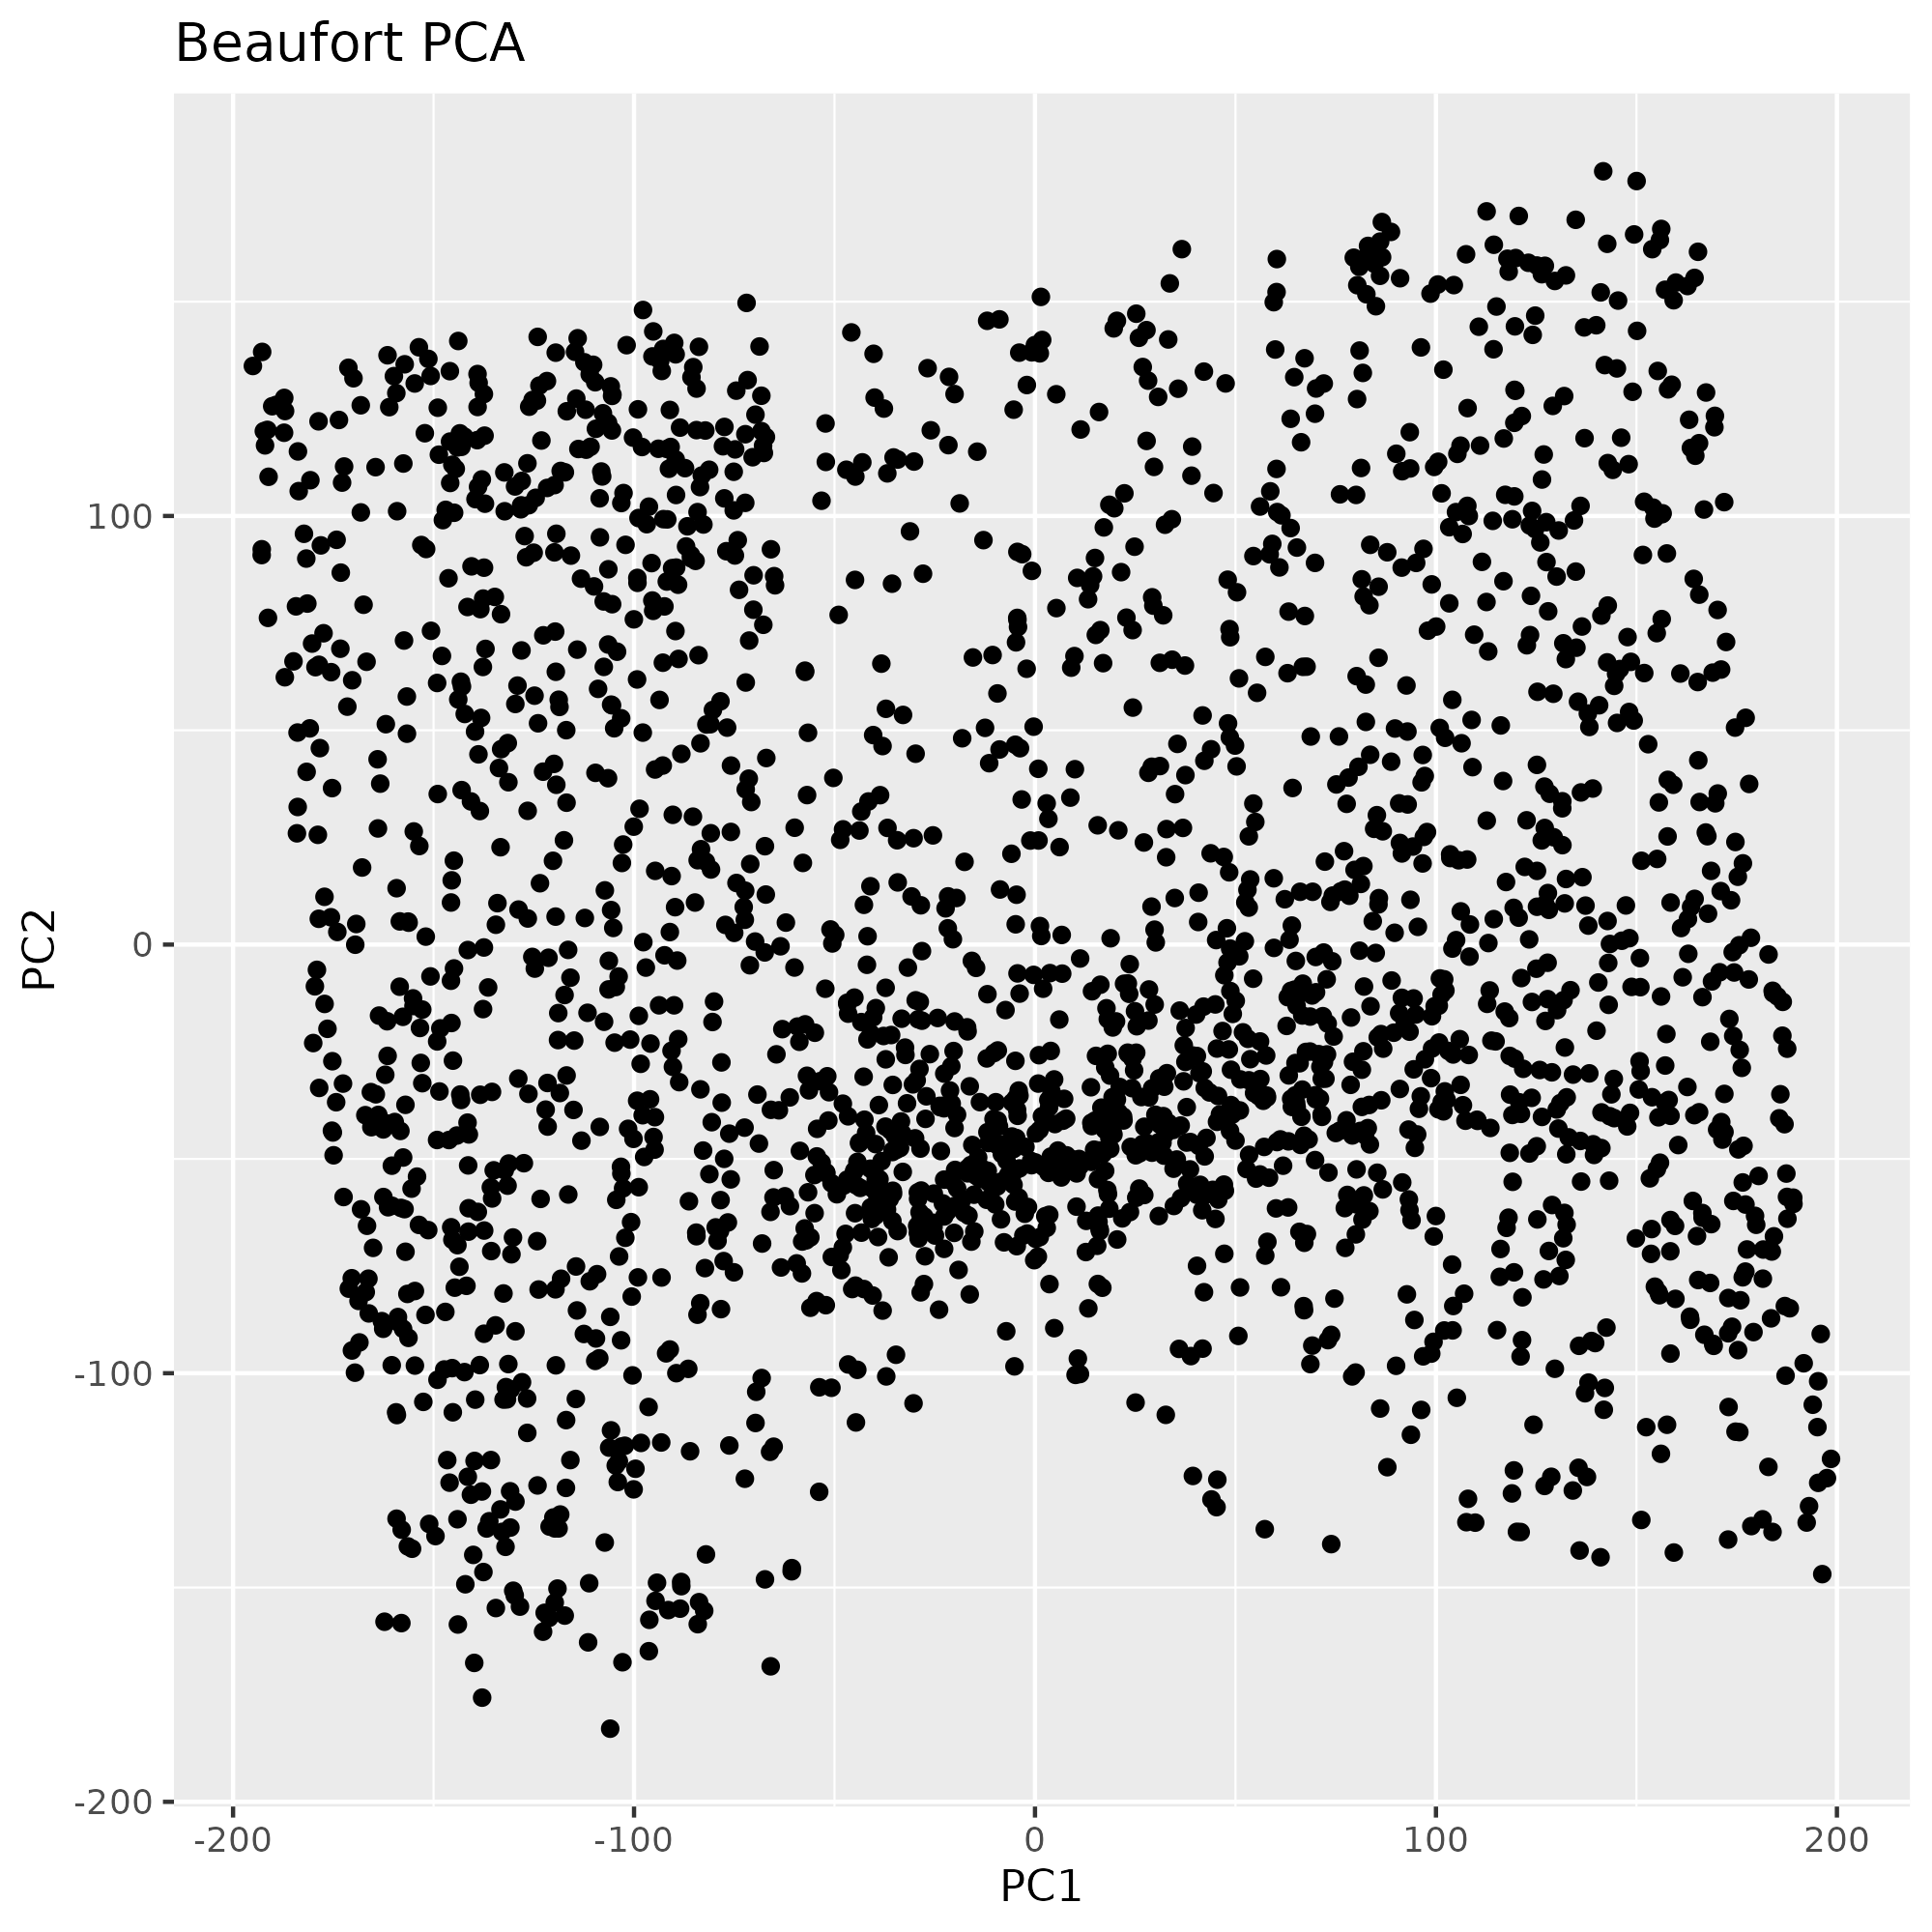
\includegraphics{figures/beaufpca.png}
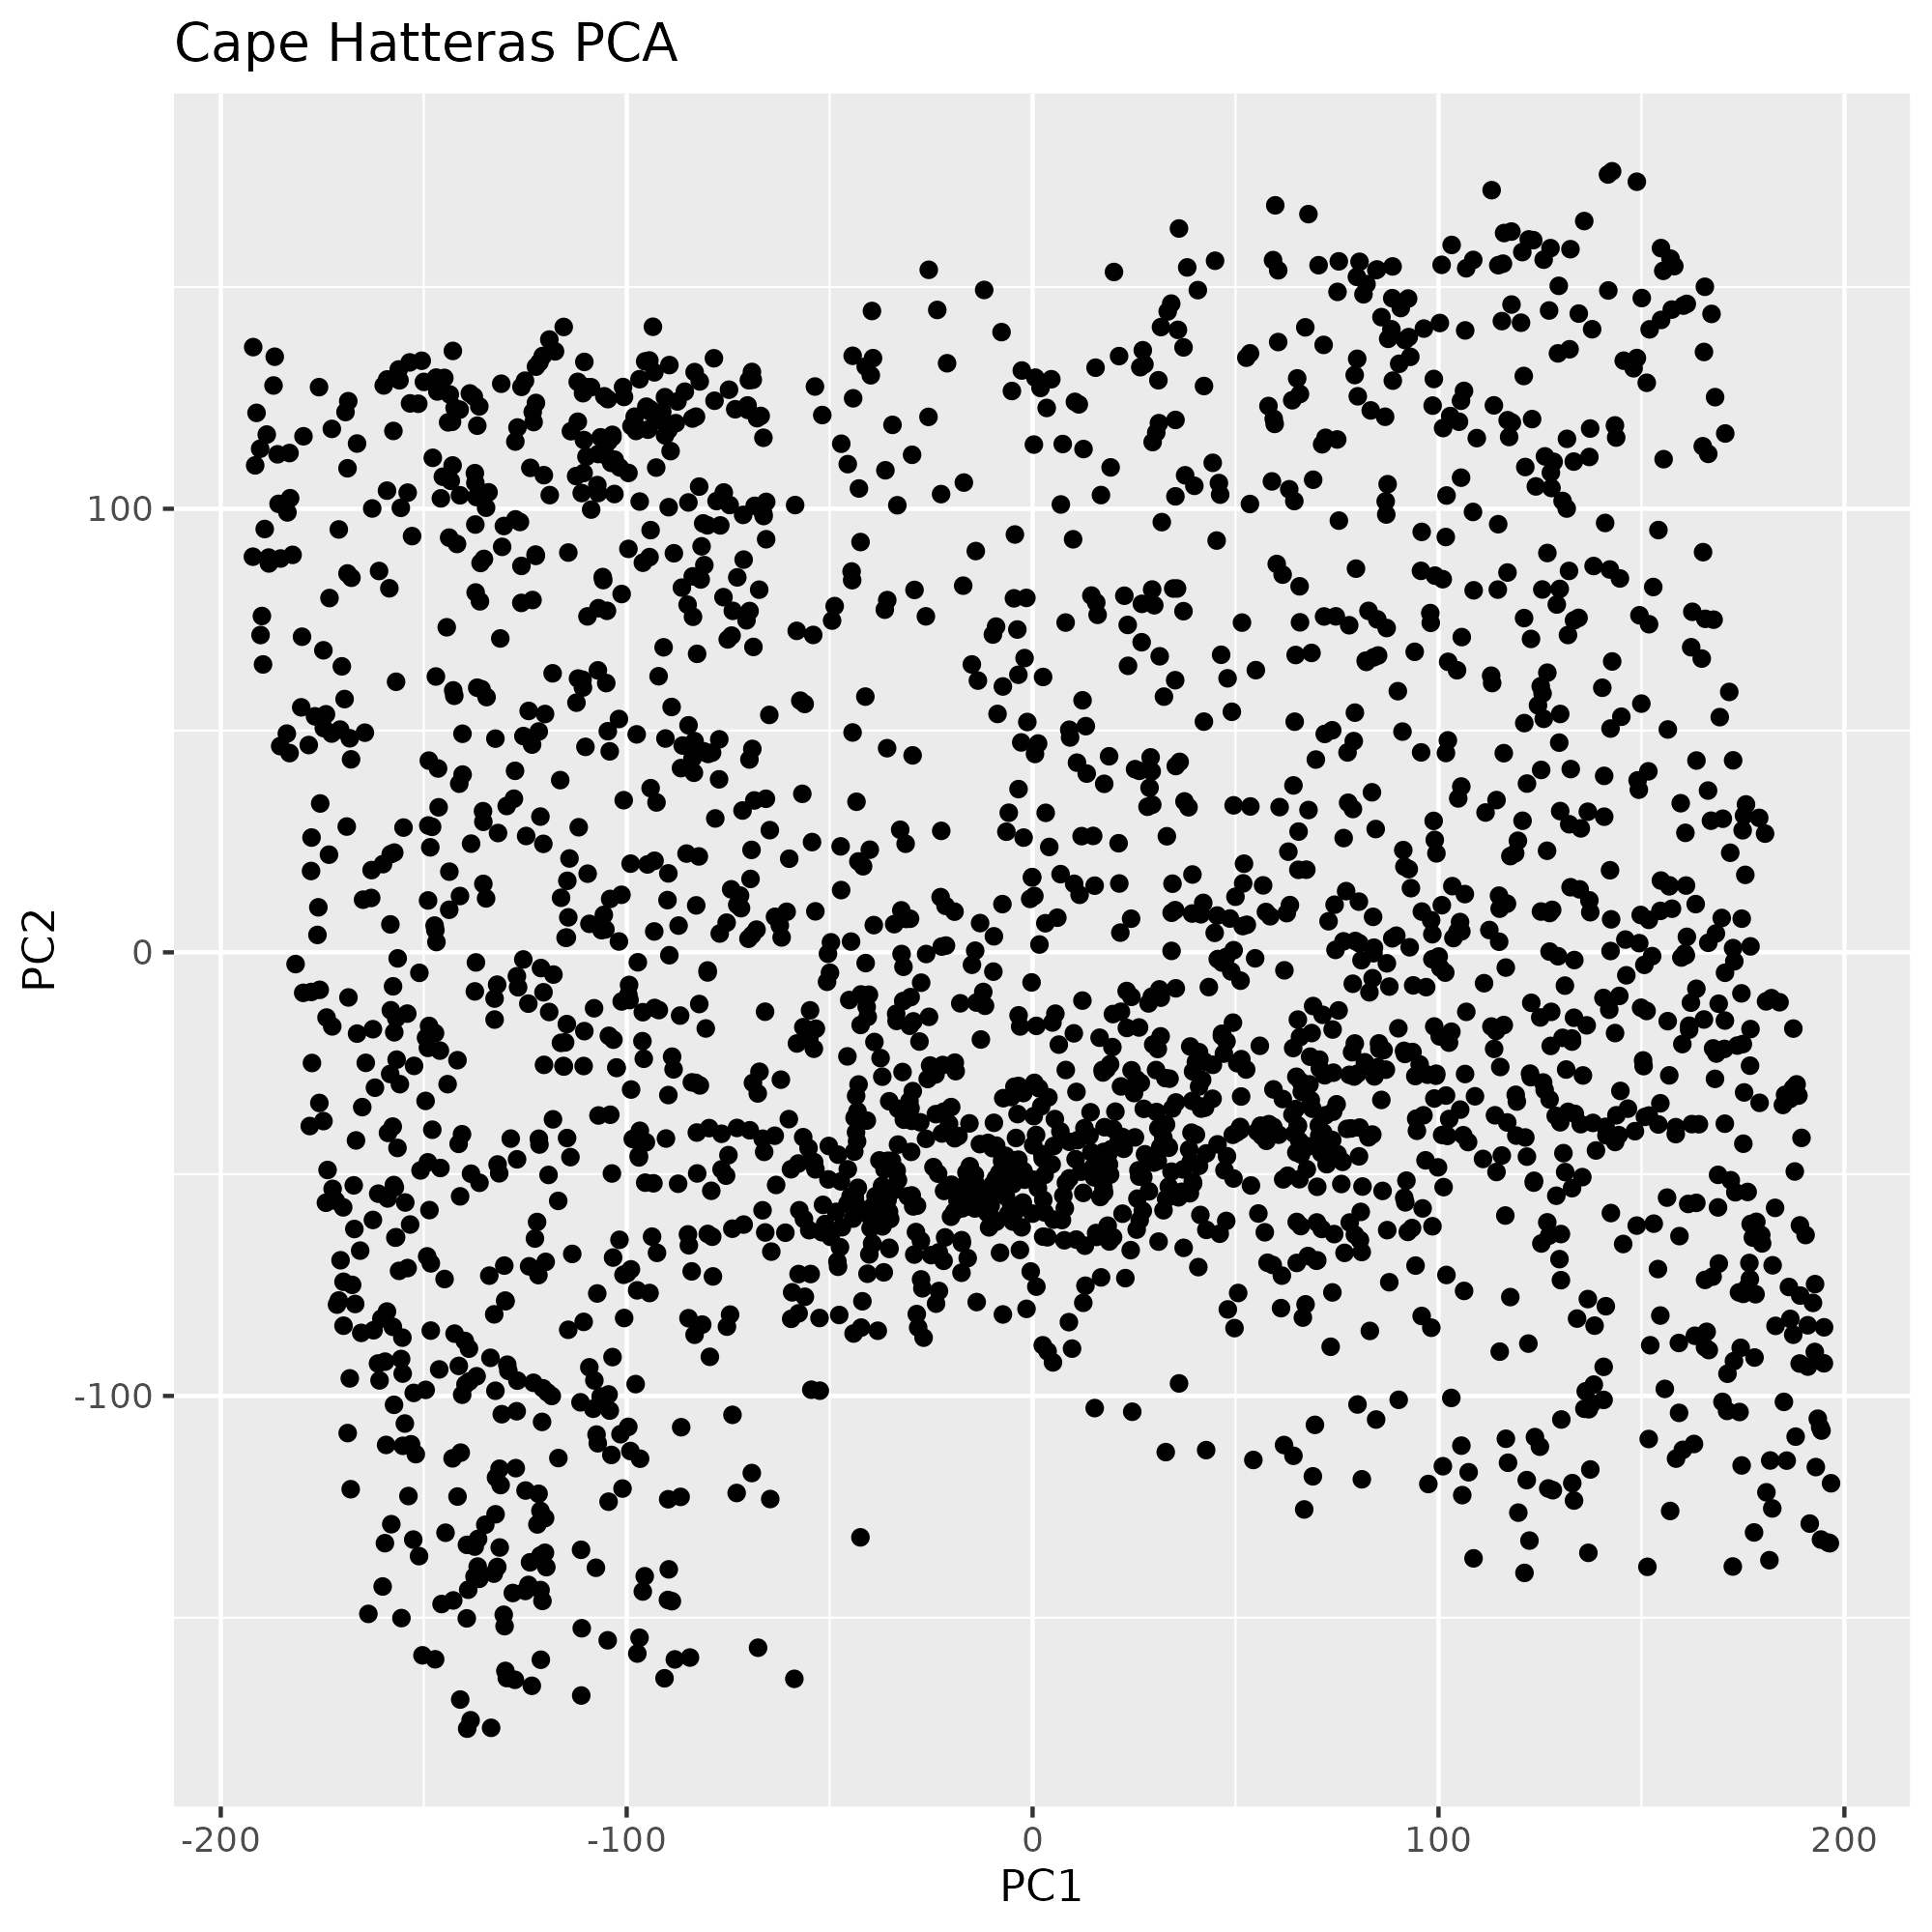
\includegraphics{figures/chpca.png}
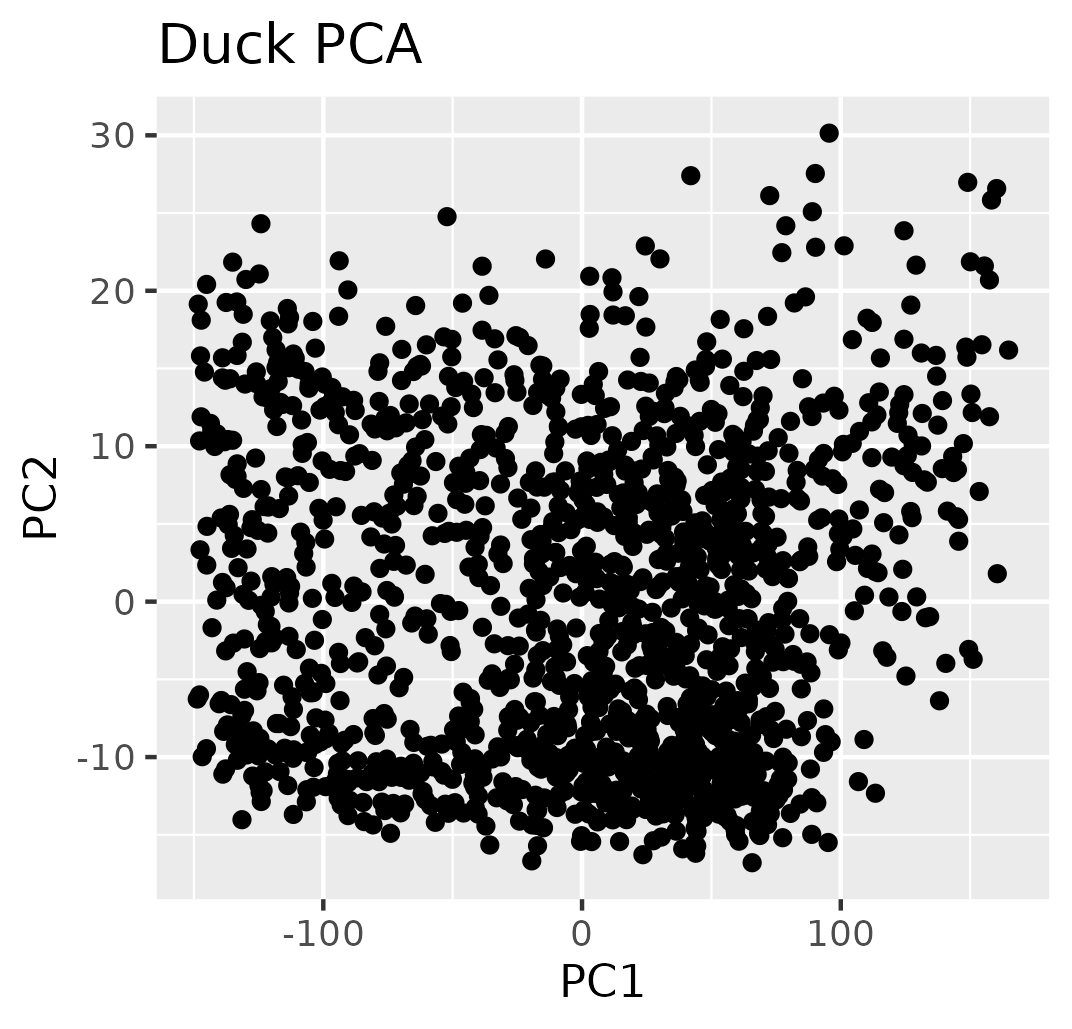
\includegraphics{figures/duckpca.png} PCA for each buoy site. There seem
to be at least one cluster in each site. From the summary table, two
components explain \textasciitilde99\% of the variance (after removing
latitude, longitude, and month) Next steps may include a clustering
analysis.

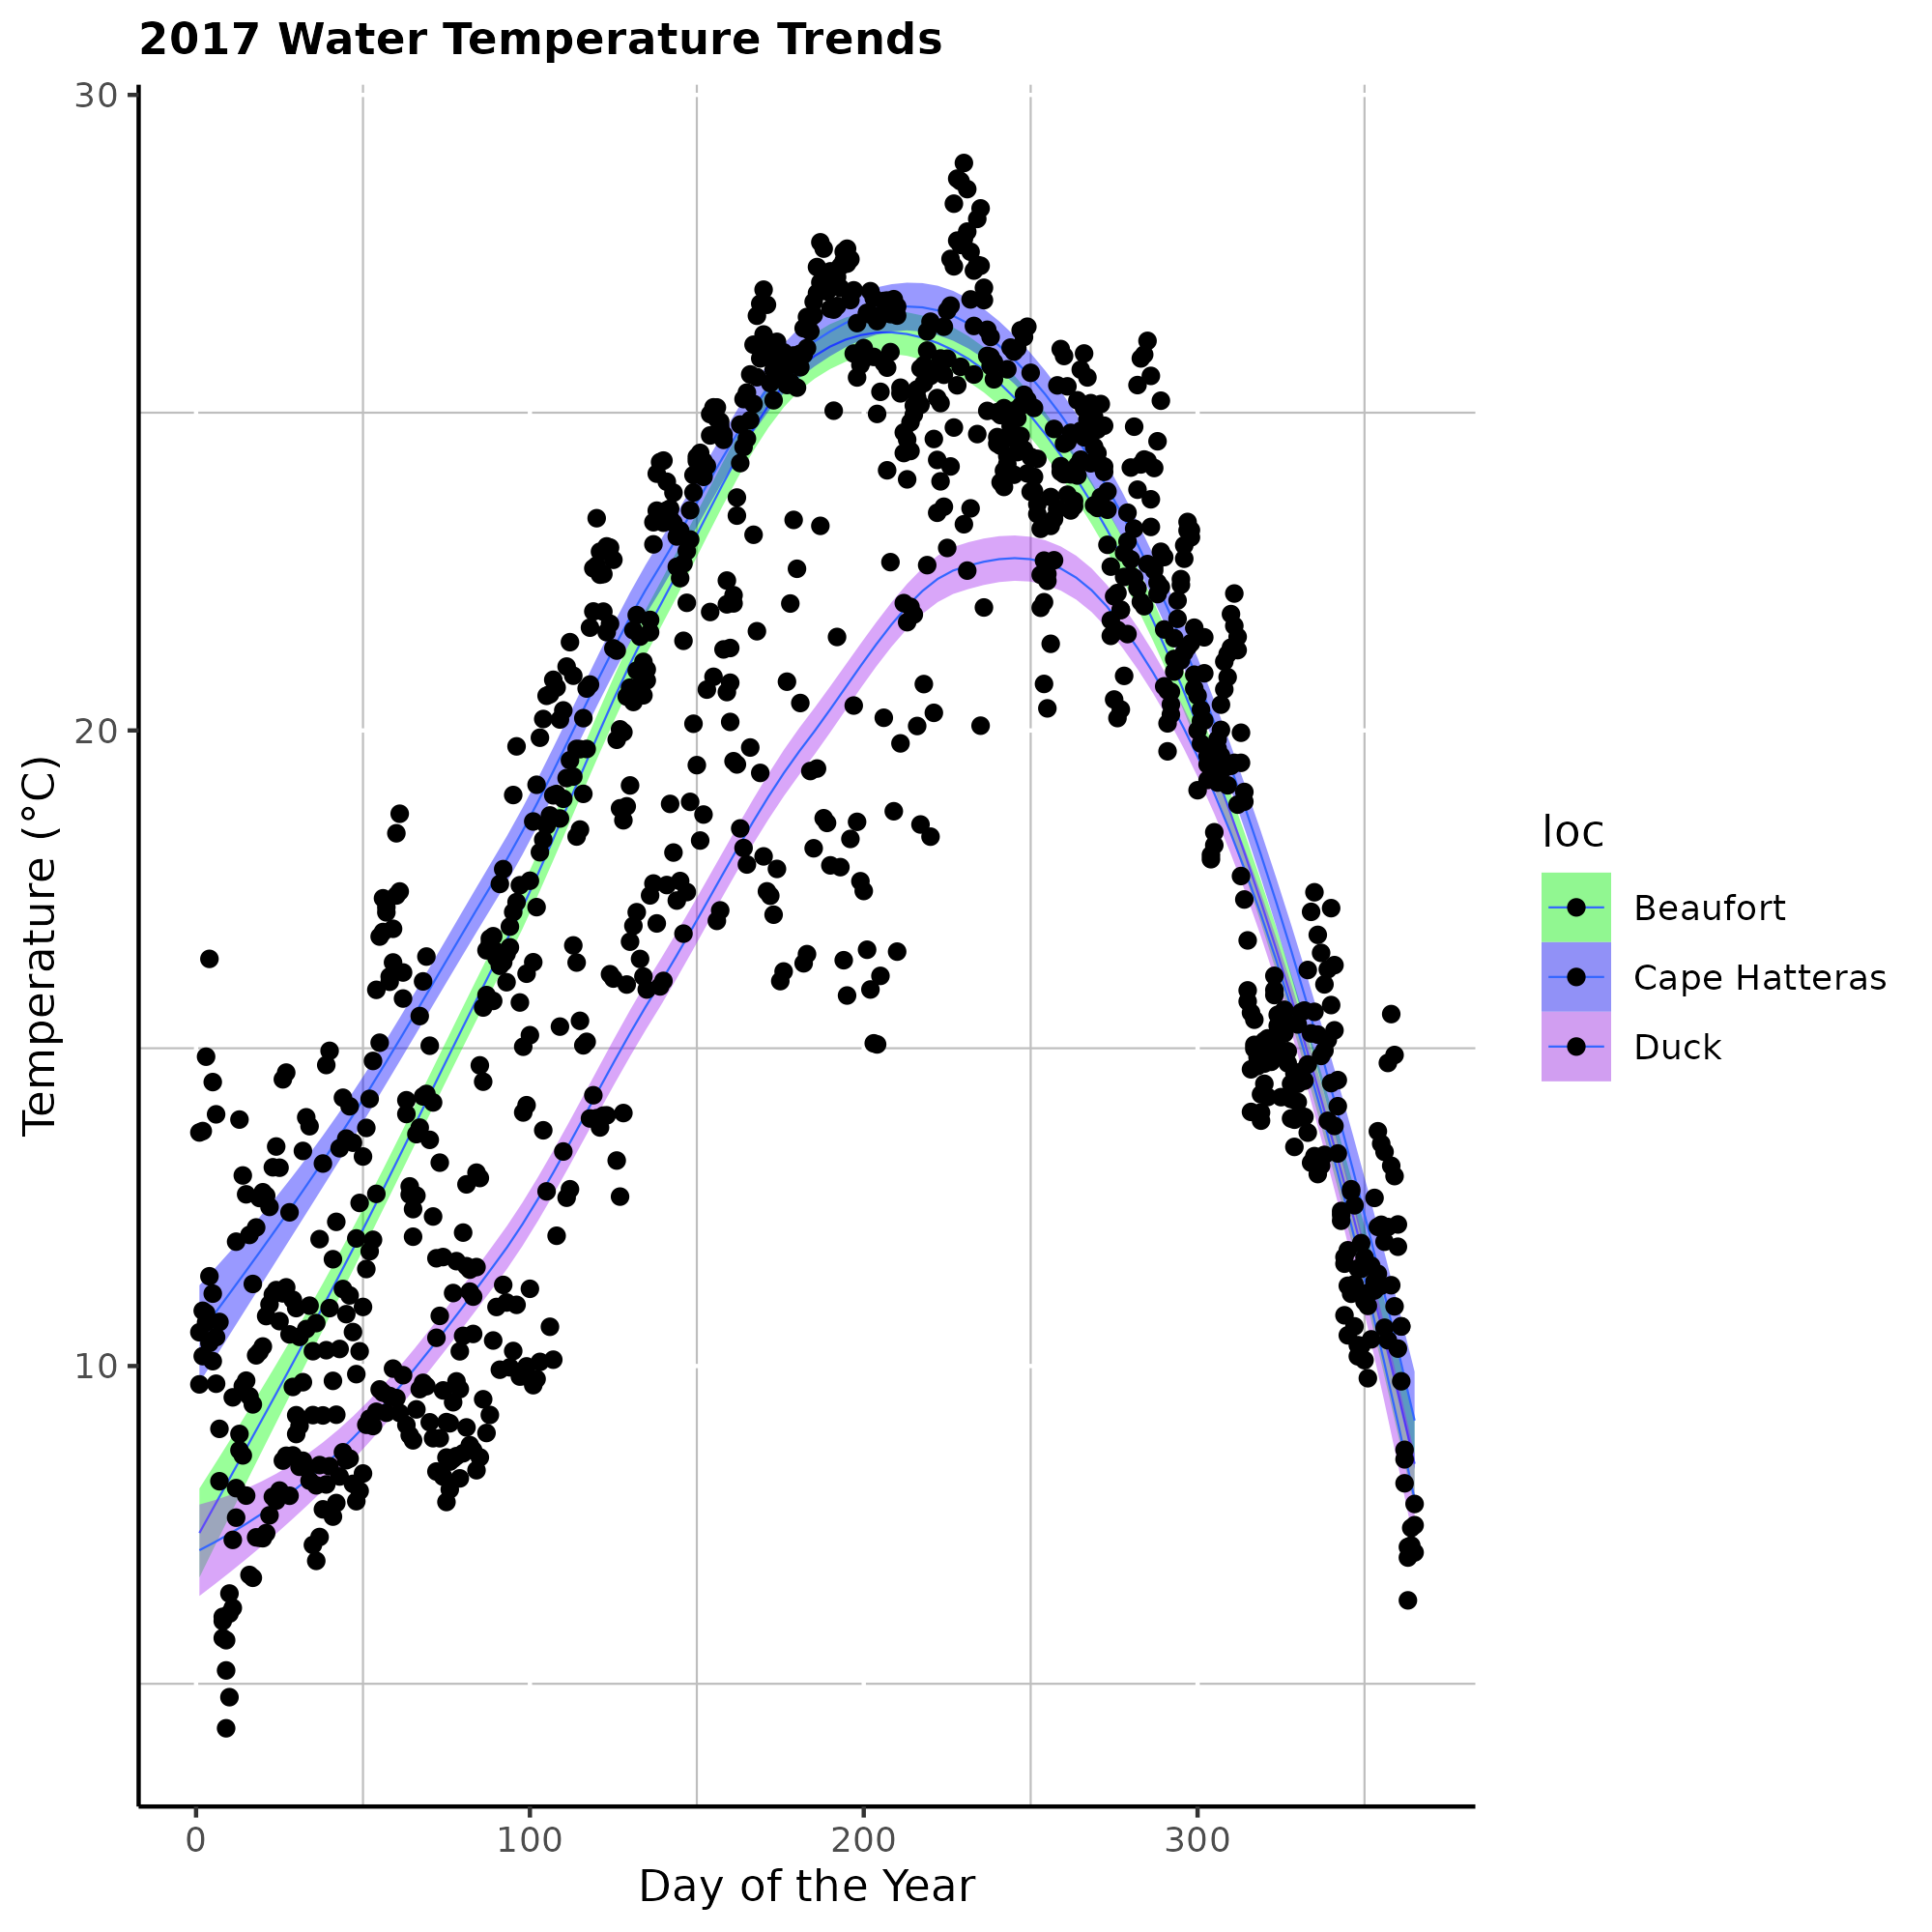
\includegraphics{figures/2017trend.png} To address the warming in 2017,
there doesn't seem to be any obvious trends. Next steps include looking
into sattelite data/literature to narrow down when the warm core ring
would have been present.

\end{document}
